\section{Index Construction}
\label{preprocessing}


As the decentralized search relies on the index structure to find paths, the constructed indexes serve as a crucial factor for accurate approximations. Previous works have studied various landmark selection strategies which have a significant impact on the accuracy of online query. In our study, we observe that even with the same landmark set, choosing which shortest path from each vertex to landmark to be indexed also plays an important role for the accuracy of online search. In this section, we propose a heuristic index construction algorithm that can generate an index that can lead to higher accuracy for decentralized search.

\begin{figure*}[ht]
    \centering
    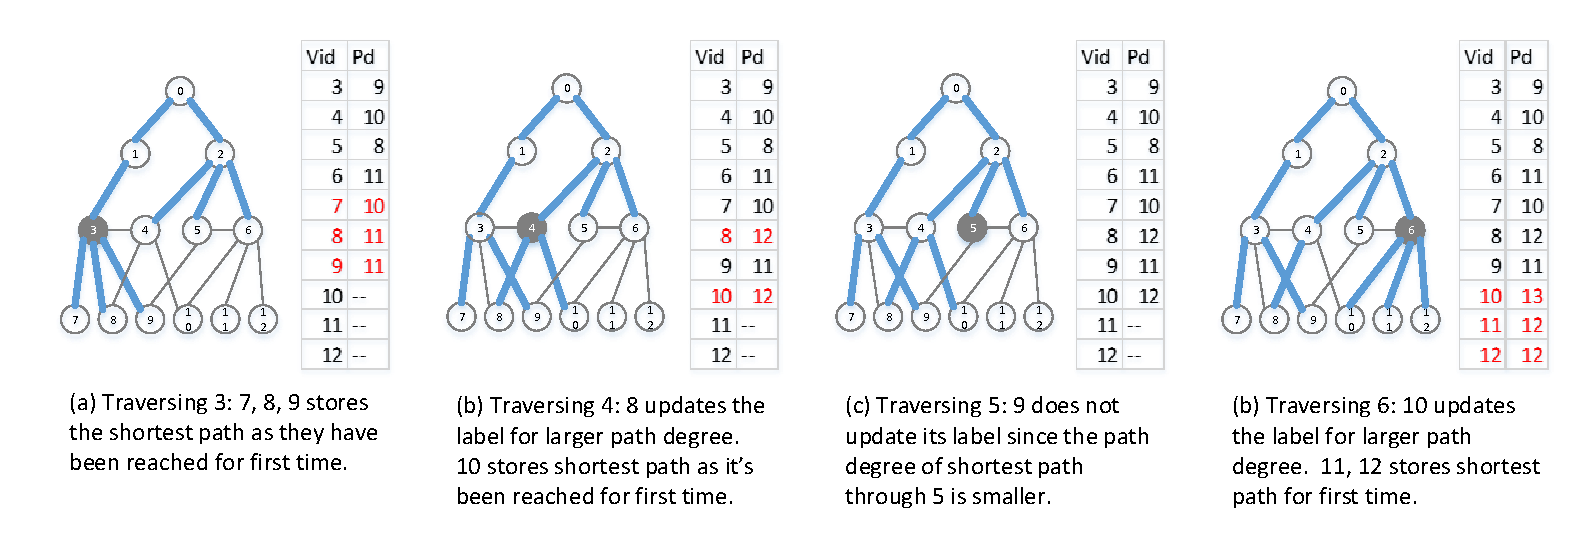
\includegraphics[width=\linewidth]{./figures/new_illustrate/bfs_illustrate.pdf}
    \caption{Heuristic algorithm that index shortest path with highest path degree during breadth first search}
    \label{fig:bfs_illustrate}
\end{figure*}

\subsection{Heuristic index construction algorithm}
\begin{algorithm}
    \caption{Algorithm heuristic index construction vertex program running on $u$}
		\label{alg:ind}
    \begin{algorithmic}
				\Function{Index construction}{$root$}
					\State $PD \gets \emptyset$
					\State $L \gets \emptyset$
					\State $Q \gets \emptyset$
					\State $L[root.id] = root.id$
					\State $PD[root.id] = root.degree$
					\State $Q.push(root)$
					\While{$Q \neq \emptyset$}
						\State $u = Q.pop()$
						\For{$each v adjecent to u$}
							\If{$v.id \not \in L$}
								\State $L[v.id] = L[u.id] \cup v.id$
								\State $PD[v.id] = PD[u.id] + u.degree$
								\State $Q.push(v)$
							\ElsIf{$L(v).size() < L(u).size() + 1$}
								\State $continue$
							\ElsIf{PD[v.id] < PD[u.id] + u.degree}
								\State $L[v.id] = L[u.id] \cup v.id$
								\State $PD[v.id] = PD[u.id] + u.degree$
							\EndIf
						\EndFor
					\EndWhile
					\State \Return $L$
        \EndFunction
    \end{algorithmic}
\end{algorithm}

[need improvement of the writing here]
On the core of decentralized search is to find neighbor vertices that share LCA with target vertex at a higher level of the indexed shortest path tree. From the point of view of a vertex, a good shortest path from each landmark to be indexed should be the one that intersects with most of other shortest paths. So that the average chance to find a shorter path from other vertices to it is higher. For each vertex, we want to find a shortest path that has common ancestors with the largest number of other vertices to be indexed. So we are actually looking for the shortest path which intersects with most other paths to increase the chance for decentralized search to find a shorter path from other vertices to this one.

We propose a greedy heuristic to construct an index which can lead to better accuracy in online queries. For each vertex $u$, when generating a label for it to store a shortest path to landmark $l$, we want to store the one that has vertices with highest betweeness centrality, i.e. intersects with most other shortest paths. Since it is quite costly to calculate the betweeness centrality, we use the degree of each vertex along the shortest path as a approximation which is much easier to compute. We call this value the path degree $Pd$. Path degree can be easily calculated by summing up the degree of vertices along the path.

The calculation of path degree can be easily embedded into the BFS during index construction. The path degree of shortest path follows optimal substructure, i.e. if $(u, .., w, ..., v)$ has the highest path degree among all the shortest path from $u$ to $v$, then the path degree of $(u, ..., w)$ is also the highest among all the shortest path from $u$ to $w$. For each vertex, the shortest path with highest degrees can be calculated easily by comparing path degree of indexed shortest path of its parents and selecting the highest one. Such calculation can be done during breadth first search with little overhead by caching the path degree of the label of each vertex. Fig. \ref{fig:bfs_illustrate} shows an example of how to greedily select shortest path with the highest path degree during breadth first search. When traversing vertex $4$, even though vertex $8$ has already been indexed with a shortest path $(0, 1, 3, 8)$ into its label, due to that $(0, 2, 4, 8)$ has a higher path degree, the label of vertex $8$ is updated. The same thing happens to vertex $10$ while traversing vertex $6$.
